% Chapter 1

\chapter{Supervised Learning} % Main chapter title

\label{Chapter1} % For referencing the chapter elsewhere, use \ref{Chapter1} 

%----------------------------------------------------------------------------------------

% Define some commands to keep the formatting separated from the content 
\newcommand{\keyword}[1]{\textbf{#1}}
\newcommand{\tabhead}[1]{\textbf{#1}}
\newcommand{\code}[1]{\texttt{#1}}
\newcommand{\file}[1]{\texttt{\bfseries#1}}
\newcommand{\option}[1]{\texttt{\itshape#1}}

%----------------------------------------------------------------------------------------

\section{Initial Considerations}

\begin{enumerate}
    \item Regression: Linear Regression and Generalized Linear Models (GLM's);
    \item Instance-based Algorithms: k-Nearest Neighbor (KNN);
    \item Decision Tree Algorithms: CART (Classification and regression tree);
    \item Bayesian Algorithms: Naive Bayes;
    \item Ensemble Algorithms: Random Forest, AdaBoost, eXtreme Gradient Boosting;
    \item Deep Learning Algorithms: Convolution Neural Network.
\end{enumerate}

%----------------------------------------------------------------------------------------

\section{Linear Regression}
      
    Using the classical linear regression model is justified if we can admit:
    
    \begin{enumerate}
        \item Linearity of the structure of $E(Y)$;
        \item Variance of the error is constant, $Var(Y) = \sigma^2$;
        \item Normality of the observations y's
        \item Independency of the observations y's
    \end{enumerate}
    
    If the assumptions (1) to (3) are not satisfied for the original data, a non-linear transformation of $Y$ might verify them, at least approximately.
    (The Box and Cox models class tries to transform the dependent variable to satisfy the assumptions (1) to (4))
    
    The $R^2$ (Coefficient of Determination) represents the proportion of the total variation explained by the relation of $\textbf{X}$ and $\textbf{Y}$ (regression).
    
    \begin{equation}
        R^2 = \frac{SQReg}{SQT} = 1 - \frac{SQRes}{SQT}
    \end{equation}
    
    Large values of $R^2$ indicates that the total variation of $\textbf{Y}$ is reduced by the insertion of the explanatory variables $X_1, X_2, \dots, X_p$
    Adding more explanatory variables to the model will increase the $R^2$. So, here is the $R^2_{adjusted}$, given by
    
    \begin{equation}
        R^2 = 1 - \frac{SQRes/(n-(p+1))}{SQT/(n-1)}
    \end{equation}
    
    $R^2_{adjusted}$ will increase when the explanatory variable addition reduces the $SQRes/(n-(p+1))$
    

\section{Generalized Linear Models}

Using the generalized linear model is justified if we can admit:
    
\begin{enumerate}
    \item $Y_i$'s are independent;
    \item $Y$ belongs to a exponential family $FE(\theta, \phi)$;
    \item Exists a function g (doubly differentiable and invertible) that relates the $\mu_i$ to a linear predictor $\eta_i = \beta_0 + \beta_1X_{1i} + \beta_2X_{2i}$
\end{enumerate}
    
The linear predictor can return values from $(-\infty, \infty)$. So if the response variable is in that interval, like a normal distribution and the link function is the identity, it is great! But if the response variable is always positive and if the mean is too distant from the zero, you can actually use the classical linear regression, because even though the linear predictor is able to return negative values, the mean is too distant from the zero and there are few values close to zero, it would not probably be able to predict negative values (unless in some extreme combination of covariables values).

\section{Mixture Models for Density Estimation and
Classification}

The mixture model is a useful tool for density estimation, and can be viewed
as a kind of kernel method. The Gaussian mixture model has the form

\begin{equation}
    f(x) = \sum^{M}_{m=1} \alpha_m\phi(x; \mu_m, \boldsymbol{\Sigma}_m)
\end{equation}

with mixing proportions $\alpha_m$, $\Sigma_m\alpha_m = 1$, and each Gaussian density has a mean $\mu_m$ and covariance matrix $\boldsymbol{\Sigma}_m$. In general, mixture models can use any component densities in place of the Gaussian in (6.32): the Gaussian mixture model is by far the most popular.

The parameters are usually fit by maximum likelihood, using the EM
algorithm as described in Chapter 8. 

Posso utilizar esse modelo quando há apenas uma variável em disposição? Sim e para quano tiver mais de uma também 

In the multivariate Gaussian mixture problem (see Exercise 12.9), the
“curse of dimensionality” raises its ugly head, where the number of para-
meters grows quickly with the increase in dimensionality. Although PCA
is often used as a first step to reduce the dimensionality, this does not help in mixtures problems because any class structure as exists may not be pre- served by the principal components (Chang, 1983).

\section{k-nearest neighbours (classifiers)}
These classifiers are memory-based and require no model to be fit. Given a query point $x_0$, we find the $k$ training points $x(r), r = 1, \dots,k$ closest in distance to $x_0$, and then classify using majority vote among the $k$ neighbors. Ties are broken at random. For simplicity we will assume that the features are real-valued, and we use Euclidean distance in feature space:

\begin{equation}
    d(i) = ||x(i) - x_0||
\end{equation}

Typically we first standardize each of the features to have mean zero and variance 1, since it is possible that they are measured in different units.

\section{Support Vector Machines (SVM's)}
Mostly used in classification problems. We may want to enlarge our feature space in order to accommodate a non-linear boundary between the classes. Produces nonlinear boundaries by constructing a linear boundary in
a large, transformed version of the feature space. The kernel approach that we describe here is simply an efficient computational approach for enacting this idea. What is the advantage of using a kernel rather than simply enlarging the feature space using functions of the original features, as in (9.16)? One advantage is computational, and it amounts to the fact that using kernels, one need only compute $K(x_i, x_i^{'})$ for all (n 2) distinct pairs $i, i^{'}$. This can be done without explicitly working in the enlarged feature space.
\begin{itemize}
    \item Advantages: efective tool in high-dimensional spaces, memory efficient (Since only a subset of the training points are used in the
    actual decision process of assigning new members, just these points need
    to be stored in memory and calculated upon when making decisions and versatility (Class separation is often highly non-linear. The ability to apply new kernels allows substantial flexibility for the decision boundaries, leading to greater classification performance)
    \item Disadvantages: SVMs are very sensitive to the choice of the kernel parameters and there is no direct probabilistic interpretation for group membership and the black box nature of these functions. The use of kernels to separate non-linear data makes them difficult (if not impossible) to interpret. Despite its popularity, SVM has a serious drawback, that is sensitivity to outliers in training samples. The penalty on misclassification is defined by a convex loss called the hinge loss, and the unboundedness of the convex loss causes the sensitivity to outliers.
\end{itemize}

\section{Random Forest}

The essential idea in bagging (Section 8.7) is to average many noisy but
approximately unbiased models, and hence reduce the variance. Trees are
ideal candidates for bagging, since they can capture complex interaction
structures in the data, and if grown sufficiently deep, have relatively low
bias. Since trees are notoriously noisy, they benefit greatly from the averaging. Moreover, since each tree generated in bagging is identically distributed (i.d.), the expectation of an average of B such trees is the same as the expectation of any one of them. This means the bias of bagged trees is the same as that of the individual (bootstrap) trees, and the only hope of improvement is through variance reduction. This is in contrast to boosting, where the trees are grown in an adaptive way to remove bias, and hence are not i.d.

The idea in random forests (Algorithm 15.1) is to improve
the variance reduction of bagging by reducing the correlation between the
trees, without increasing the variance too much. This is achieved in the
tree-growing process through random selection of the input variables.

Combination of many decision trees, effectively leveraging and combining the choices of many models (this technique of using a combination of models is known as \textbf{ensembling}).

Para classificação, uma medida de impureza que pode ser usada é:
\begin{itemize}
    \item Misclassification error
    \item Gini index
    \item Cross-entropy or deviance
    
\end{itemize}

Para regressão, uma medida de impureza que pode ser usada é  $SSE = \sum_{i \in S_1} (y_i - \bar(y)1)^2 + \sum_{i \in S_2} (y_i - \bar(y)2)^2$.

Out-of-Bag sample, no contexto de \textit{random forest}, consiste na observação que não foi selecionada na amostra \textit{bootstrap} utilizada por uma determinada árvore de decisão.

Out-of-Bag error, no contexto de \textit{random forest}, consiste na proporção de \textit{out-of-bag samples} incorretamente classificadas.

\section{AdaBoost}
How weights are updated in AdaBoost? Simply put, the idea is to set weights to both classifiers and data points (samples) in a way that forces classifiers to concentrate on observations that are difficult to correctly classify. This process is done sequentially in that the two weights are adjusted at each step as iterations of the algorithm proceed. 

AdaBoost is also extremely sensitive to Noisy data and outliers so if you do plan to use AdaBoost then it is highly recommended to eliminate them. AdaBoost has also been proven to be slower than XGBoost.

\section{Gradient Boosting Machine (Regression)}
We start with a leaf that is the average value of the variable we want to predict. Then we add a tree based on the Residuals, tree is scaled by a contrbution (fixed learning rate). Then we add another tree based on the new residuals and we keep adding trees based on the errors made by the previous tree.

\section{XGBoost}

XGBoost is an exceptionally useful machine learning method when you don't want to sacrifice the ability to correctly classify observations but you still want a model that is fairly easy to understand and interpret. 


XGBoost, scalable machine learning system for tree boosting, was designed to be used with large, complicated datasets. Just like Gradient Boost (unextreme), XGBost fits a Regression Tree to the residuals but uses a unique Regression Tree. Let's callt it XGBoost tree.

We prune the XGBoost tree based on the gain of the branch and a $\gamma$

$\lambda$ is a regularization parameter, which means that it is intended to reduce the prediction's sensitivity to individual observations, prevents over fitting the training data. It results in more pruning, by shrinking the Similarity Scores and it results in smaller Output Values for the leaves

There is a learning rate parameter also.

We calculate Similarity Scores and Gain to determine how to split the data and we prune the tree by calculating the differences between Gain values and a user defined Tree Complexity Parameter $\gamma$. If positive, then do not prune. If negative, then prune.

Then we calculate the Output Values for the remaining leaves.

The minimum number of Residuals in each leaf is determined by calculating something called Cover

One thing that is relatively unique about XGBoost is that it has default behavior for missing data. In Python, all we have to do is identify missing values and make sure they are set to 0

Uses the Second Order Taylor Approximation for both Regression and Classification.

For classification, the negative log-likelihood is the most commonly used loss function.

There are several different ways to calculate feature importances. By default, “gain” is used, that is the average gain of the feature when it is used in trees. Other types are “weight” - the number of times a feature is used to split the data, and “cover” - the average coverage of the feature. You can pass it with $importance_type$ argument.

%----------------------------------------------------------------------------------------

\section{Neural Networks}

\begin{figure}[H]
\centering
\caption{NeuralNetwork}
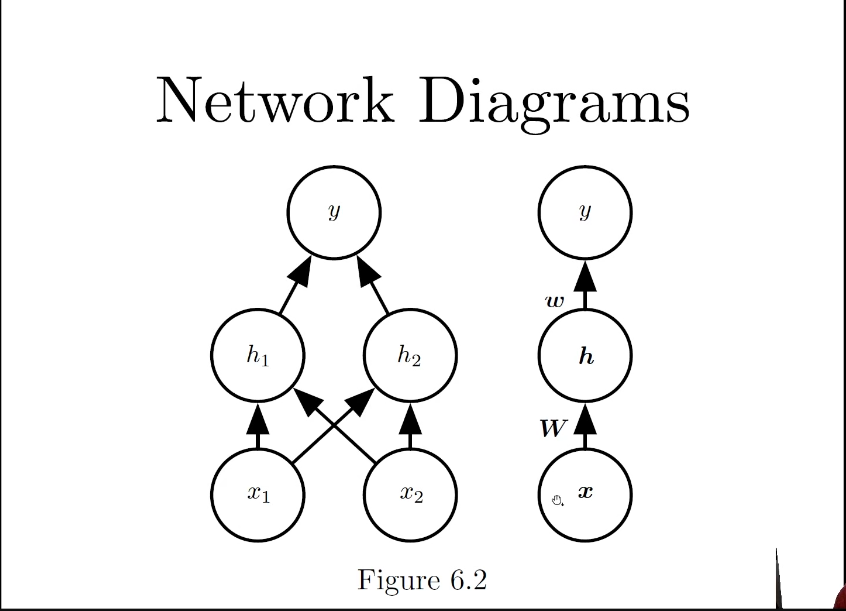
\includegraphics[scale=0.5]{Figures/network-diagram.PNG}
\end{figure}

Back-propagation is "just the chain rule" of calculus, one of the key concepts of NN. É um algortimo para calcular o gradiente de modo extramammente eficiente (baixa complexidade computacional), Is the method to calculate the gradient of the loss function with respect to the weights in an artificial neural network

\begin{enumerate}
    \item Forward prop: start an the input x, apply the weight and biases and compute y and the cost
    \item Back prop: based on the  associated y and cost, update weighs and biases?
    \item
\end{enumerate}

When we use a feedforward neural network to accept an input $\boldsymbol{x}$ and produce an
output $\hat{\boldsymbol{y}}$, information flows forward through the network. The inputs x provide
the initial information that then propagates up to the hidden units at each layer
and finally produces $\hat{\boldsymbol{y}}$ . This is called forward propagation . During training,
forward propagation can continue onward until it produces a scalar cost $J (\boldsymbol{\theta})$.
The back-propagation algorithm,  often simply called backprop, allows the information from the cost to then flow backwards through
the network, in order to compute the gradient.


The term back-propagation is often misunderstood as meaning the whole
learning algorithm for multi-layer neural networks. Actually, back-propagation refers only to the method for computing the gradient

Activating functions: the softmax function is used as the activation function in the output layer of neural network models that predict a multinomial probability distribution. That is, softmax is used as the activation function for multi-class classification problems where class membership is required on more than two class labels.

\section{Time Series Models}
Para verificar o poder preditivo do modelo é interessante comparar as métricas de performance do modelo proposto com as de um \textit{naive forecast model} (benchmarking)

\subsection{ARMA}
Modelos ARMA só podem ser aplicados para séries estacionárias. No
entanto, a maior parte das séries não são estacionárias.
\subsection{ARIMA}
Um modelo ARMA Integrado, ARIMA(p,d,q), consiste em aplicar o
modelo ARMA(p,q) na d-ésima diferença da série. Aplicar d-diferenças torna a série estacionária. Geralmente d = 1 ou d = 2 é suficiente para séries não sazonais (ou com sazonalidade ajustada)
\subsection{SARIMA}
\subsection{ARIMAX}
\subsection{SARIMAX}

\section{Conceitos importantes}

\subsection{Multicolinearidade}
Multicollinearity happens when independent variables in the regression model are highly correlated to each other. It makes it hard to interpret of model and also creates an overfitting problem. It is a common assumption that people test before selecting the variables into the regression model. How to check wheter Multicollinearity occurs?

\begin{enumerate}
    \item Plot the correlation matrix of all the independent variables
    \item Use the Variance Inflation Factor (VIF) for each independent variable. It is a measure of multicollinearity in the set of multiple regression variables. The higher the value of VIF the higher correlation between this variable and the rest.
\end{enumerate}

How to fix the Multi-Collinearity issue?
\begin{enumerate}
    \item Variable selection
    \item Variable transformation
    \item PCA (Principal Component Analysis): the character of variable independence
\end{enumerate}

\subsection{Cross Validation}
Consiste em dividir o conjunto de dados (treino + teste) em $k$ pedaços. Em seguida, para cada combinação de $k-1$ pedaços, é ajustado o modelo de interesse e calculado, no pedaço restante, a(s) métrica(s) de validação. Útil para comparar a performance entre modelos distintos e para selecionar os melhores  \textit{tunning parameters}. Algumas variações desse procedimento:

\begin{enumerate}
    \item \textbf{K-Fold Cross Validation}
    \item \textbf{Leave One Out Cross Validation}
    \item  \textbf{Repeated Cross Validation}
\end{enumerate}

\subsection{Bagging (Boostrap Aggregating)}
Dado um conjunto de dados de treino, o procedimento \textit{bagging} gera novas $m$ amostras com reposição desse conjunto (esse tipo de amostra é chamada de \textit{bootstrap}), para, em seguida, ajustar $m$ modelos nas $m$ amostras \textit{bootstrap} (um modelo para cada amostra) e combinar o output em uma média (no caso de regressão) ou votação (no caso de classificação). The essential idea in bagging is to average many noisy but approximately unbiased models, and hence reduce the variance. The number of trees B is not a critical parameter with bagging; using a very large value of B will not lead to overfitting. In practice we use a value of B sufficiently large that the error has settled down.

\begin{figure}[H]
\centering
\caption{Illustration of bagging}
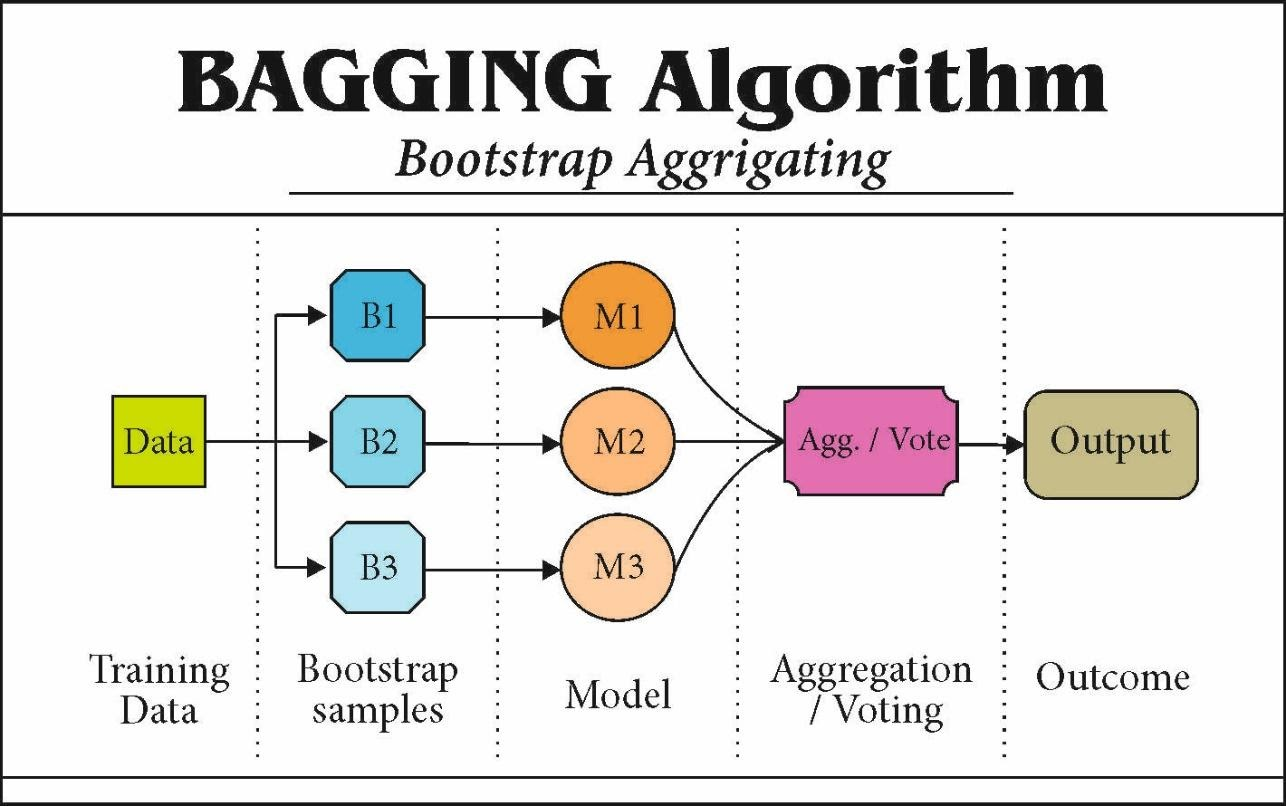
\includegraphics[scale=0.2]{Figures/bagging.jpg}
\end{figure}


\subsection{Boosting}
A weak classifier is one whose error rate is only slightly better than
random guessing. The purpose of boosting is to sequentially apply the
weak classification algorithm to repeatedly modified versions of the data,
thereby producing a sequence of weak classifiers $G_m(x)$, $m = 1, 2,\dots, M$.

Boosting works in a similar way of the bagging procedure except that the trees are grown sequentially: each tree is grown using information from previously grown trees. Boosting does not involve bootstrap sampling; instead each tree is fit on a modified version of the original data set. Boosting has three parameters:

\begin{enumerate}
    \item The number of trees B. Unlike bagging and random forests, boosting can overfit if B is too large, although this overfitting tends to occur slowly if at all. We use cross-validation to select B.
    
    \item The shrinkage parameter $\lambda$, a small positive number. This controls the rate at which boosting learns. Typical values are 0.01 or 0.001, and the right choice can depend on the problem. Very small $\lambda$ can require using a very large value of B in order to achieve good performance.
    
    \item The number $d$ of splits in each tree, which controls the complexity of the boosted ensemble. Often $d$ = 1 works well, in which case each tree is a stump, consisting of a single split. In this case, the boosted ensemble is fitting an additive model, since each term involves only a single variable. More generally $d$ is the interaction depth, and controls the interaction order of the boosted model, since $d$ splits can involve at most $d$ variables.
\end{enumerate}

\subsection{Regularization}
Regularized regression consists in estimating a penalized function of the form.

\begin{equation}
\underset{f \in H}{min} \Big[ \sum_{i = 1}^{N}
L(y_i, f(x_i)) + \lambda J(f) \Big ], 
\end{equation},

where $L(y, f(x))$ is the chosen loss function, $J(f)$ is a penalty functional and $H$ is a space of function on which $J(f)$ is defined (Hastie, Tibshirani, and Friedman, 2009)

Produces models that are more parsimonious and have similar prediction error as the full model and it is usually robust enough to not be influenced by the correlated variables. 
    
For tree-based methods, there is not yet a well established regularization procedure in the literature.

\begin{enumerate}
\item \textbf{Ridge Regression (L2)}: consiste em adicionar uma penalidade equivalente aos quadrados das magnitudes dos coeficientes, na função de custo. É útil para fazer \textit{shrink} das estimativas dos parâmetros (pode chegar perto de zero, mas não exatamente 0) e reduzir a complexidade do modelo e a multicolinearidade. Conforme \textit{Introduction to Statistical Learning}, tem-se que \textit{it is best to apply ridge regression after standardizing the predictors}.

When the number of variables $p$ is almost as large as the number of observtions $n$, the OLS estimates will be extremely variable. And if $p > n$, then the OLS estimates do not even have a unique solution, whereas ridge regression can still perform well by trading off a small increse in bias for a large decrease in variance (bias and variance tradeoff)

\item \textbf{Lasso  Regression (L1)}: consiste em adicionar uma penalidade equivalente às magnitudes dos coeficientes, na função de custo. É útil para reduzir \textit{overfitting} e selecão de variáveis (os coeficientes podem chegar a zero). Sendo assim, resulta em uma equação mais imples e mais fácil de interpretar.

\item \textbf{Regularization Elastic Net}: consiste em uma combinação entre \textit{Ridge Regression (L1)} e \textit{Lasso Regression (L2)}. Pode ajudar a excluir certos parâmetros.
\end{enumerate}

\subsection{Métricas de avaliação}
\subsubsection{Regressão}

\begin{enumerate}
    \item Mean Squared Error (MSE):
    
    \begin{equation}
        MSE = \frac{1}{n}\sum^n_{i=1}(Y_i - \hat{Y}_i)^2
    \end{equation}
    
    Like variance, mean squared error has the disadvantage of heavily weighting outliers.[11] This is a result of the squaring of each term, which effectively weights large errors more heavily than small ones. This property, undesirable in many applications, has led researchers to use alternatives such as the mean absolute error, or those based on the median. 
    \item Mean Absolute Error (MAE)
    \item Mean Absolute Percentage Error (MAPE)
\end{enumerate}

\subsubsection{Classificação}

\begin{table}[H]
\centering
\caption{Matriz de Confusão}
\begin{tabular}{@{}cc cc@{}}
\multicolumn{1}{c}{} &\multicolumn{1}{c}{} &\multicolumn{2}{c}{\textbf{Predição}} \\ 
\cmidrule(lr){3-4}
\multicolumn{1}{c}{} & 
\multicolumn{1}{c}{} & 
\multicolumn{1}{c}{False (-)} & 
\multicolumn{1}{c}{True (+)} \\ 
\cline{2-4}
\multirow[c]{2}{*}{\rotatebox[origin=tr]{0}{\textbf{Classe}}}
& False (-) & TN (True Negative) & FP (False Positive) \\[1.5ex]
& True (+) & FN (False Negative)   & TP (True Positive) \\
\cline{2-4}
\end{tabular}
\label{confusion-matrix}
\end{table}

\begin{align*}
\text{Accuracy} &= \frac{TN + TP}{TN + FP + FN + TP}\\
\text{Precision} &= \frac{TP}{TP + FP}\\
\text{Recall, Sensitivity, True Positive Rate} &= \frac{TP}{TP + FN}\\
\text{F1 Score} &= 2\frac{precision * recall}{precision + recall}\\
\end{align*}

É interessante fazer a Curva ROC, gráfico entre \textit{True Positive Rate} e \textit{False Positive Rate} (FP / (FP + TN)). It summarizes all of the confusion matrices that each threshold produced.

A utilização da acurácia não é recomendado no caso de um conjunto de dados desbalanceados.

